\documentclass{proc}
\usepackage{graphicx}
\graphicspath{ {./images/} }

\begin{document}
	
	\title{CS573 Spring 2022 Final Project Process Book}

	
	\author{Truman Larson}
	
	\maketitle
	
	\section{Overview and Motivation}
		\begin{figure} [t]
			\centering
			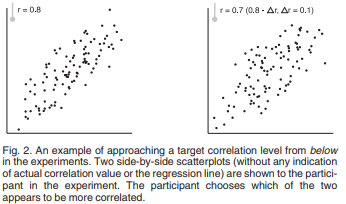
\includegraphics[width=0.5\textwidth]{methods}
			\caption{Methods used by Yang}
			\label{fig:methods}
		\end{figure}
		Animation in visualization is an area that has been criticized as a ineffective method of conveying information \cite{Robertson2008}. Realistically, animation is a tool just like any other, and has its good and bad use cases. One opportunity is in the area of visualization judgment, specifically in correlation. Some visual features have already been identified and evaluated \cite{Yang2019}, but there remains an opportunity to explore other types of features, specifically animated ones. The goal of this project is to take the first few steps in that direction and explore the potential and challenges of animation visualization, while also creating a tool that can assist with understanding what correlation visualization methods work well together. Eventually, this work could be adapted into an experiment, like the one shown in figure \ref{methods}, to determine the validity of animation in correlation judgment and to see specifically what methods work the best. For now, creating a robust, expandable, and intuitive tool is the priority. 
		
	\section{Related Work}
		\begin{figure}[t]
			\centering
			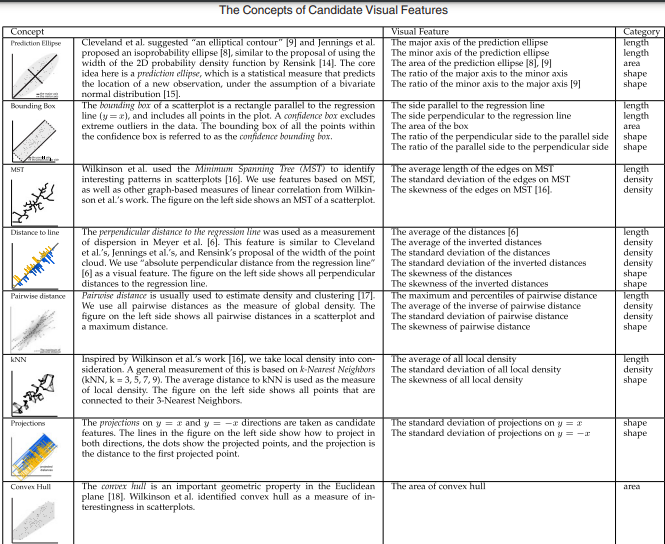
\includegraphics[width=0.5\textwidth]{concepts}
			\caption{List of conceptual visual features Yang theorized for how we perceive correlation in scatterplots.}
			\label{fig:concepts}
		\end{figure}
		Figure \ref{fig:concepts} shows a list of visual figures developed by Yang et al. \cite{Yang2019}. This work is the main basis for this project and their evaluation of these visual features proved invaluable. The main gap in the utilization of these features is the fact that they are static. Larsen et al. provides context as to how people compare patterns and suggests that mental translation may be a significant factor \cite{larsen1998effects}. Thus, including animation in the list of visual features serves only to complete the list. 
	\section{Questions}
		\begin{itemize}
			\item Does animated feedback improve individuals' performance in correlation judgement?
			\subitem While the scope of this question is broad, it is ultimately what this project is working towards. Overtime, this question was narrowed to the specific details of implementation and feasibility, but this remained the penultimate goal throughout. 
			\item What animation types are best for reinforcing correlation perceptual ideas?
			\subitem As seen in Larsen et al., metal translation was a good starting point for answering this question. Again, as I moved forward with this project, it became more a question of feasibility and implementation.
			\item What visual features work well together?
			\subitem This is what I believe is the core question that this project specifically is trying to answer. Giving a platform to judge and play with different combinations of animation and visual features will give a platform for future work. 
		\end{itemize}
	\section{Data} 
		While this project doesn't specifically use a data source, it is worth mentioning that all of the data used in the charts, and the charts themselves, are generated using code provided by Lane Harrison and Yiren Ding. The code provides a way to generate data that has a particular correlation coefficient. This data can easily be displayed using the chart code they provided as well.
	\section{Exploratory Data Analysis}
		Since there is no data to analyze really, this section is mainly going to be looking at the original designs used by Yang et al. 
		\begin{figure}[t]
			\centering
			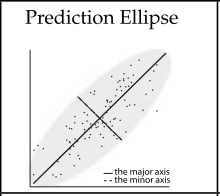
\includegraphics[width=0.2\textwidth]{ellipse}
			\caption{Ellipse visual feature example \cite{Yang2019}}
			\label{fig:ellipse}
		\end{figure}
		\begin{figure}[t]
			\centering
			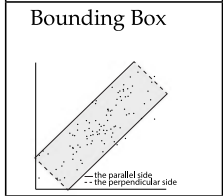
\includegraphics[width=0.2\textwidth]{bounding}
			\caption{Bounding box visual feature example \cite{Yang2019}}
			\label{fig:bounding}
		\end{figure}
		\begin{figure}[t]
			\centering
			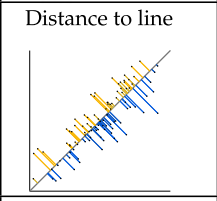
\includegraphics[width=0.2\textwidth]{distance}
			\caption{Distance to line visual feature example \cite{Yang2019}}
			\label{fig:distance}
		\end{figure}
		\begin{figure}[t]
			\centering
			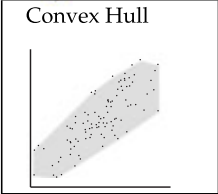
\includegraphics[width=0.2\textwidth]{convex}
			\caption{Convex hull visual feature example \cite{Yang2019}}
			\label{fig:convex}
		\end{figure}
		Figures \ref{fig:bounding} through \ref{fig:convex} were the best performing figures outlined by Yang et al. Out of these features, I was personally drawn towards the ellipse as a feature due to its simplicity and visually appealing nature. The distance to line does seem helpful, but would need significant efforts to de-clutter to make more intuitive. I see the idea behind the bounding box, but it just seems way too clunky to be useful. The convex hull was the one that confused me the most, but I can see its usefulness. 
		
		The other big aspect that these designs revealed to me was the necessity of a trendline in these types of graphs. It gives a really good reference to compare each point to and provides a bit more context that I think would be useful in any chart. 
	
	\section{Design Evolution}
		After the initial evaluation of the designs, I designed and implemented the prediction ellipse and the bounding box with Madyson Kelly in place of my Assignment 3. The aspects of the feedback design themselves were quite simple as they were clearly defined, though the implementation was a bit less straight forward. The important part of the design was the application itself. When first designing this tool, we emphasized the importance of a few key aspects: modularity, expandability, and ease of use. The application has to be modular so that many different combinations can easily be tested and judged. A modular application would mean maximizing the reusuability of the individual parts, making the level of "mix and match" that we wanted possible. Expandability is an important aspect since we initially did not know how many different types of charts we would want and what add on features we would end up needing. Making an application that was modular and expandable meant that these parts could be added on easily with minimal editing. Lastly, we wanted to emphasize the ease of use of the tool. Making it easy to use gives more motivation to try more types of combinations. If we make it ugly and unintuitive, no one would even want to use it making it useless. 
	
		Next, we evaluated what animation and add-on features would best fit the application. As mentioned before, translation of the elements is a base animated feature we wanted to try. The best way to do this, however, was not as clear. Initially, we thought to combine the two charts and simply change the color so that the user could compare one color to the other. While this does work, it still is very cluttered and hard to read. Later in the project, I got some better advice to make the comparison an active process, having the user click to highlight one chart or the other. This proved to be much more helpful overall. 
		
		Moving through the experiment, I found that most people I asked to check out my project would tilt their head to view the comparison. This prompted similar research into rotation, but none such research was easily found. However, rotating the charts such the theoretical trendline was horizontal proved to be much easier to read and compare, especially when the two charts were combined. 
		
		This project does deviate from the proposal greatly. This was mainly an issue of scope since the proposal describes a full experiment that would not have been possible. The scope was shrunk to just lay the groundwork for an experiment of that nature. 
	\section{Implementation}
		\begin{figure}[t]
			\centering
			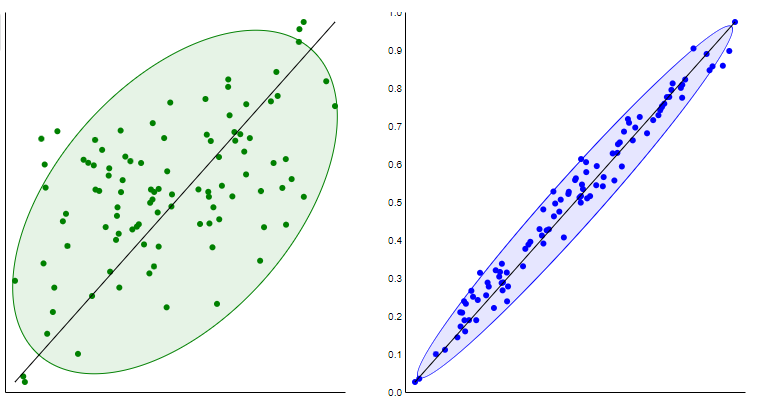
\includegraphics[width=0.2\textwidth]{ellipse-final}
			\caption{Ellipse visual final implementation}
			\label{fig:ellipse-final}
		\end{figure}
		\begin{figure}[t]
			\centering
			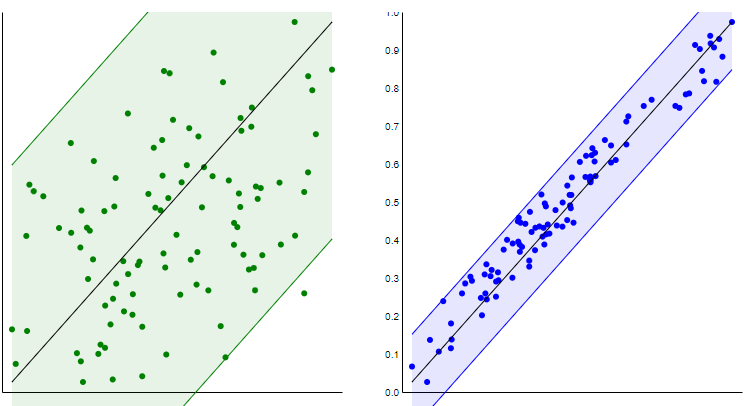
\includegraphics[width=0.2\textwidth]{bounding-final}
			\caption{Bounding box final implementation}
			\label{fig:bounding-final}
		\end{figure}
		\begin{figure}[t]
			\centering
			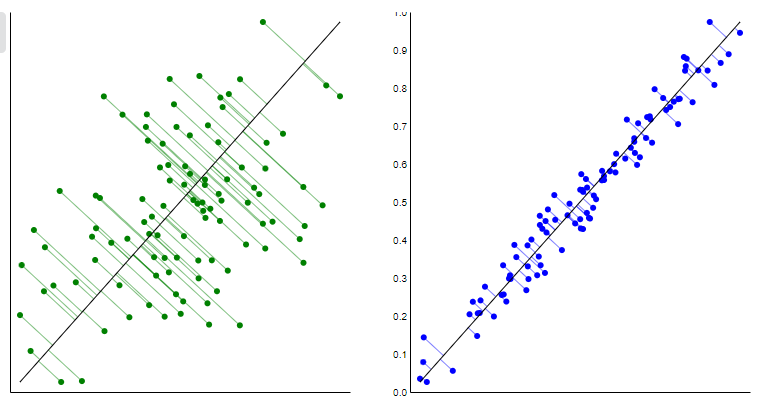
\includegraphics[width=0.2\textwidth]{distance-final}
			\caption{Distance to line final implementation}
			\label{fig:distance-final}
		\end{figure}
		\begin{figure}[t]
			\centering
			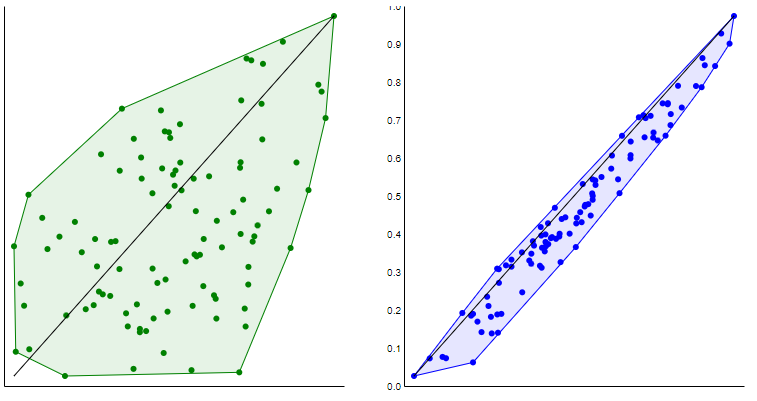
\includegraphics[width=0.2\textwidth]{convex-final}
			\caption{Convex hull final implementation}
			\label{fig:convex-final}
		\end{figure}
		
		For the final charts shown in figures \ref{fig:ellipse-final} through \ref{fig:convex-final}, the implementation was mostly hindered by technical details rather than design. Much of the time was spent figuring out exactly how to get the features in the correct spot such that the visualization was accurate. Some of the visualization had algorithms provided to us. The ellipse algorithm was given by Lane Harrison provided in turn by the authors of Yang et al. Additionally, the convex hull algorithm found online and provided by Project Nayuki (https://www.nayuki.io/page/convex-hull-algorithm). 
		
		A large part of the implementation was also spent realizing the design principles planned out in the previous section. Each chart is in its own file, and each add on also resides in its own file. There is a simple method for passing information about the underlying charts between each of the functions. 
		
		Most of the charts also have some element of animation build in within them. This was mainly for aestetic purposes. The add-on, like the trendline and axis fade, are also animated for this reason.
		
		\begin{figure}[t]
			\centering
			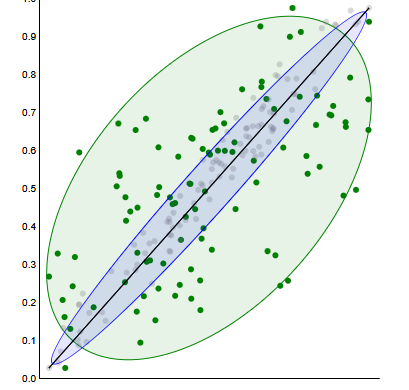
\includegraphics[width=0.2\textwidth]{merge}
			\caption{Merge final implementation}
			\label{fig:merge}
		\end{figure}
		\begin{figure}[t]
			\centering
			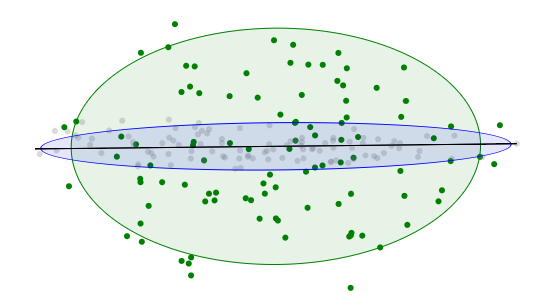
\includegraphics[width=0.2\textwidth]{merge-rotate}
			\caption{Merge and rotate final implementation}
			\label{fig:merge-rotate}
		\end{figure}
	
		The core animations, shown in their completion in figures \ref{fig:merge} and \ref{fig:merge-rotate} were relatively trivial to implement using d3 animations. As figure \ref{fig:merge-rotate} shows, having both of the animations together results in a clear and easy comparison. 
		
		\begin{figure}[t]
			\centering
			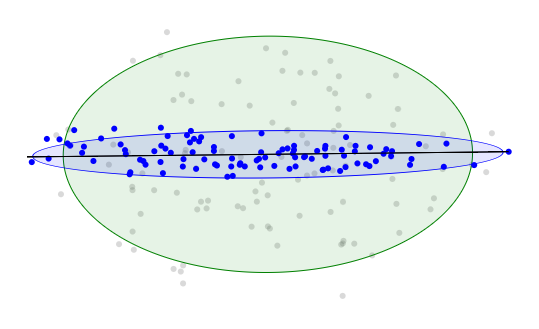
\includegraphics[width=0.2\textwidth]{toggle}
			\caption{Toggle declutter final implementation}
			\label{fig:toggle}
		\end{figure}
		
		One of the final core features is the toggle feature. This isn't very obvious at first, but one the user is used to the website, it becomes a valuable tool for decluttering the graphs after merging. This is on by default whenever the graphs are merged together and clicking them will toggle which graph is highlighted by changing the color and opacity. 
		
		\begin{figure}[t]
			\centering
			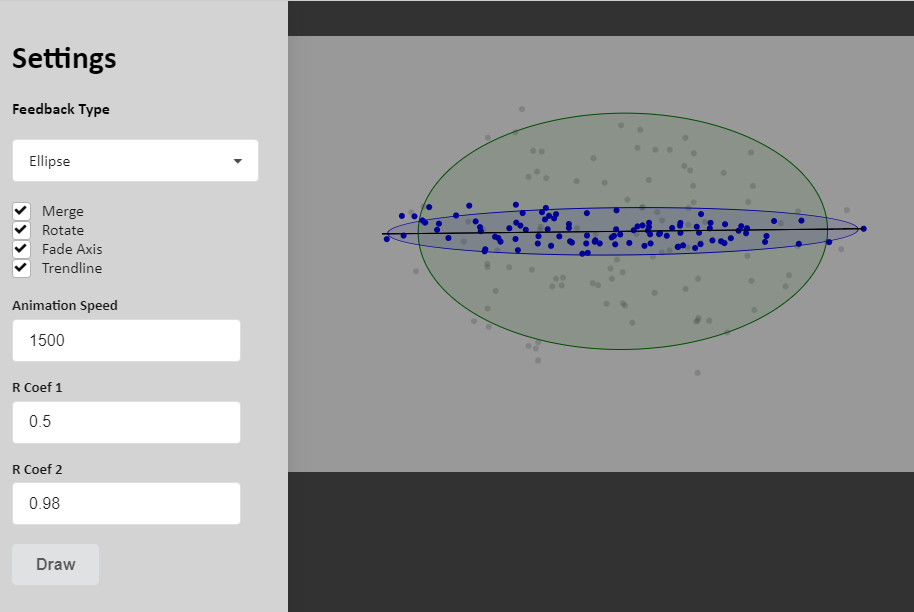
\includegraphics[width=0.5\textwidth]{ui}
			\caption{Settings user interface final implementation}
			\label{fig:ui}
		\end{figure}
		
		The most important aspect is the actual interface that changes all of the settings that are implemented. For the UI design, I utilized components and styling provided by semantic-ui. Figure \ref{fig:ui} shows the settings available to the user. The user can change the type of chart, any of the add on feature, the animation speed, or the R coefficients. Making this pleasing to the eye and easy to use was extremely important. Thus, I utilized as many resources as were available to make it both visually and interactively appealing. 
		
	\section{Evaluation}
		
		This visualization accomplishes the final questions we had of "What visual features work well together?". Through even my own experiences developing, and with the small amount of features currently available, I found that merging and rotating makes things easier to compare. Though I also found that decluttering is vital to making this work. Additionally, the value of trendline for visualizations was enormous since it was a consistent reference point that I was able to use personally to evaluate them at times. It worked especially well with the ellipse since it gave a good reference to where the center of the ellipse was. Looking through all the combinations, I can easily see what works and what doesn't and I feel like that alone accomplishes what we set out to do. The obvious step now is adding both more visual and interactive features. Increasing the amount of combinations that either I or another user could make exponentially increases the value of this tool. Specifically, I think that making the animations more interactive, such as a playback feature where the user can scrub through the steps of the animation, would be incredibly valuable. Simply put, the more features that are added to this, the more value it can give. 

	

	\bibliographystyle{abbrv}
	\bibliography{prospectus}
\end{document}